\documentclass[pdf]{beamer}
% Berlin Berkeley Warsaw
\newcommand\go[1]{\texttt{#1}}
\usepackage{listings}
\usepackage{xeCJK}
\lstset{
	language=Go,
	basicstyle=\ttfamily,
	keywordstyle=\color{blue}\ttfamily\bfseries,
	identifierstyle=\color{green!70!black},
	commentstyle=\ttfamily\color{gray},
	stringstyle=\ttfamily\color{red},
	showstringspaces=true
}
\mode<presentation>{\usetheme{Berlin}\useoutertheme{infolines}\useinnertheme{rounded}}
\title{A Whirlwind Tour of Go}
\subtitle{Just the Cool Parts}
\author{Steve Willoughby}
\begin{document}
\begin{frame}
	\titlepage
	\begin{center}
	
\includegraphics[height=.25\textheight]{go-logo}
	
\includegraphics[height=.25\textheight]{gopher}
	\end{center}
\end{frame}
\section[Overview]{Overview}
\subsection{What Are We Doing Here?}
\begin{frame}{The Point}
	\begin{itemize}
		\item ``What \emph{is} Go?''
		\item ``What is it actually good for?''
		\item ``Why should I care?''
	\end{itemize}
\end{frame}
\subsection{Motivation for Go}
\begin{frame}{30 Seconds of History}
	\begin{itemize}
		\item Designed by Rob Pike, Ken Thompson, and Robert Griesemer.
		\item Includes direct experience with C from day 1 to now.
			\pause
		\item ``If we were to design C today, knowing what we know now, on today's technology\dots''
			\pause
			\begin{itemize}
		\item $\therefore$ Go's syntax is very much like C's
		\item \dots\ but cleaned up and streamlined a bit.
			\end{itemize}
		\pause
		\item Dreamed up while waiting on a 45-minute C++ compile
		\pause
			\begin{itemize}
				\item Fast compilation
				\item Native binary compiler with low overhead
				\item Strong static typing
				\item Extraordinarily spartan
			\end{itemize}
	\end{itemize}
\end{frame}
\subsection{The Basics of Go}
\begin{frame}[fragile]{Go Syntax}
	\begin{itemize}
		\item Type declarations \emph{follow} identifier names
\begin{lstlisting}
var x int
var UserName string

func AddNumbers(x, y int) int { ... }
func DivideNumbers(x, y int) (int, error) { ... }

type Shape struct {
   X     int
   Y     int
   Color ColorCode
}
\end{lstlisting}
	\end{itemize}
\end{frame}
\begin{frame}{Program Structure}
	\begin{itemize}
		\item Basic unit is a \emph{package} (namespace boundary).
		\item Multiple source files in a package, in the same directory tree.
		\item Every program must have a \go{main} package.
		\item The \go{main} package has a \go{main} function.
		\item Import packages into the program using the \go{import} statement.
		\item Always prefix identifiers from imported packages with their package name.
		\item Identifiers can be \emph{public} or \emph{private} w/r/t package boundaries.
			\begin{itemize}
				\item Identifier names starting with an uppercase letter are public.
				\item All others are private.
			\end{itemize}
	\end{itemize}
\end{frame}
\begin{frame}[fragile]{Hello, World}
\begin{lstlisting}
/* Standard-issue "Hello, World" program in Go */
package main

import "fmt"

func main() {
     fmt.Println("Hello, 世界")
}
\end{lstlisting}
\end{frame}
\subsection{The Go Ecosystem}
\begin{frame}{The Playground}
	\begin{itemize}
		\item Interactive playground to immediately try something in Go.
		\item \go{https://go.dev/play/}
	\end{itemize}
	\begin{center}
		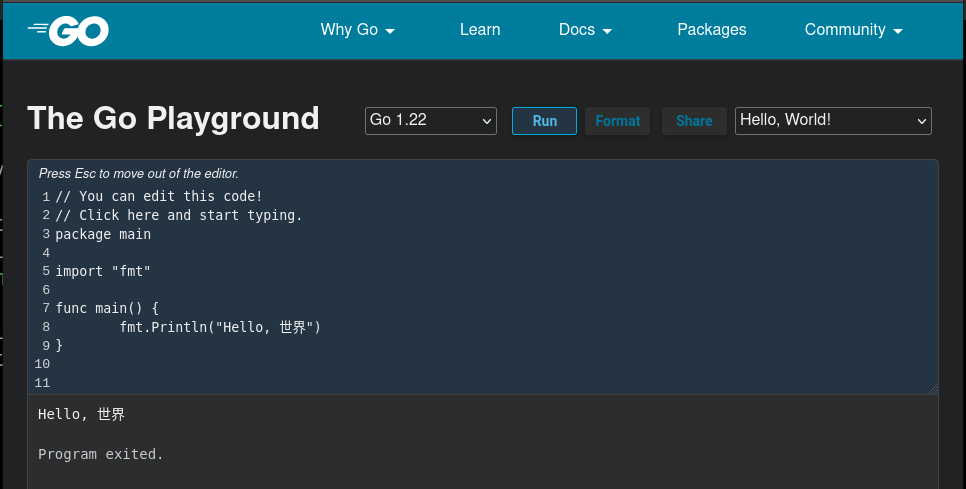
\includegraphics[width=\textwidth]{playground}
	\end{center}
\end{frame}
\begin{frame}[fragile]{Importing Third-Party Packages}
	\begin{itemize}
		\item Standard library package names are simple names:
			\begin{lstlisting}
import "fmt"
import "encoding/json"
import "flag"
import "math"
\end{lstlisting}
	\end{itemize}
	\vfill
	\strut
\end{frame}

\begin{frame}[fragile]{Importing Third-Party Packages}
	\begin{itemize}
		\item Standard library package names are simple names:
\begin{lstlisting}
import (
   "fmt"
   "encoding/json"
   "flag"
   "math"
)
\end{lstlisting}
\pause
		\item Getting packages from public repositories:
			\pause
\begin{lstlisting}
import "github.com/MadScienceZone/go-gma/v5/dice"
\end{lstlisting}
	\end{itemize}
	\vfill
	\strut
\end{frame}
\begin{frame}{Automatic API Documentation}
\begin{itemize}
\item\go{https://pkg.go.dev/}\emph{repository-url}
\end{itemize}
	\begin{center}
		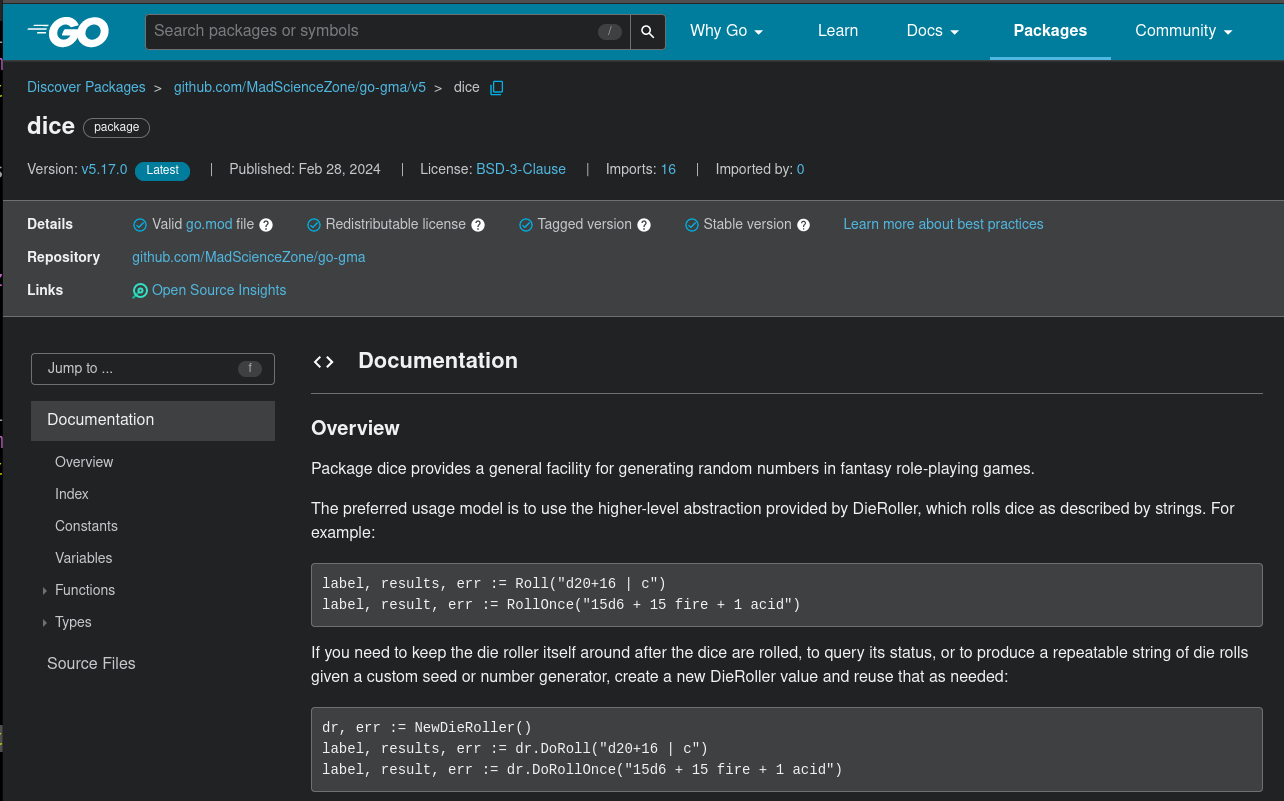
\includegraphics[width=\textwidth]{docsite}
	\end{center}
\end{frame}



\end{document}
